\documentclass[11pt]{article}

\usepackage[margin=0.92in]{geometry}
\usepackage{amsmath,amssymb,booktabs,tabularx,array,xcolor,float}
\usepackage{graphicx}
\graphicspath{{figures/}}
\usepackage[round]{natbib}
\usepackage[colorlinks=true,citecolor=blue!45!black,urlcolor=blue!45!black]{hyperref}
\usepackage{microtype}

\setlength{\parindent}{0pt}
\setlength{\parskip}{0.45em}
\setlength{\emergencystretch}{3em}

\title{Calibration\\
\large Equivalence-scale specification: revised calibration section}
\author{Tommaso De Santo}
\date{}

\begin{document}
\maketitle

\section{Two Changes to the Model}
\label{sec:changes}

Two changes relative to the model section of the circulated draft matter for
the calibration.

First, children no longer enter through the committed consumption and housing
bundles $(\bar c(n,s),\bar h(n,s))$ of the draft. Within-period utility for a
household with $n$ dependent children at home is
\begin{equation}
u(c,h,n)
=
\frac{\left(c^{\alpha(n)}\,h^{1-\alpha(n)}/e(n)\right)^{1-\sigma}}{1-\sigma}
+\psi\,n,
\qquad
\alpha(n)=\alpha_0-\left(\delta_{\mathrm{jump}}\mathbf 1\{n\geq1\}+\delta_a n\right),
\label{eq:eqscale_utility}
\end{equation}
where $e(n)=((2+0.7n)/2)^{0.7}$ is the equivalence scale of
\citet{scholzSeshadriKhitatrakun2006}, imposed rather than estimated, and
normalized to one for a childless couple. The household evaluates the
consumption--housing composite per equivalent adult: children lower flow
utility at a given bundle and raise the marginal value of the composite
through $e(n)$, and they tilt spending toward housing through $\alpha(n)$,
both only while they live at home. Households without children at home have
the homothetic preferences of the childless, and $\psi$ is the direct utility
flow per child at home. There are no minimum-consumption or minimum-housing
requirements, which is what permits empirical income risk below.

Second, fertility is sequential rather than one-shot. Each period during the
fertile ages, a childless household chooses between waiting and trying for a
first birth, and a household with $n<3$ children and a child still at home
chooses between stopping and trying for child $n+1$. An attempt at age $a$
succeeds with the fecundity probability
\begin{equation}
\pi_a=1-0.02\,e^{0.134\,(a-18)}
\quad\text{for } a<45,
\qquad
\pi_a=0 \text{ thereafter},
\label{eq:fecundity}
\end{equation}
which declines from $0.98$ at age 18 to $0.50$ at age 42.\footnote{The two
coefficients are set so that the four-year success probability tracks the
age profile of natural fecundability in \citet{leridon2004}. They imply
four-year probabilities of about $0.90$, $0.80$, and $0.62$ at ages 30, 35,
and 40, against Leridon's estimates of $0.91$, $0.84$, and $0.64$ for a
conception leading to a live birth within four years. A least-squares fit to
the full schedule is pending.} Completed family size is therefore an outcome
of starting age,
biology, and sequential choices; no household ever chooses a number of
children. Both decisions carry type-1 extreme-value taste shocks, with scale
$\kappa_E$ on the entry decision and $\kappa_C$ on the continuation decision.
The two scales are allowed to differ because the two decisions are different
objects: the timing of the first attempt depends on circumstances the model
does not describe, such as partnership timing and career events, so
$\kappa_E$ can be large, while the continuation decision of an established
family should be governed by prices, income, and preferences, so $\kappa_C$
is expected to be small.

\section{Calibration}
\label{sec:quant_calibration}

I organize the model parameters into two groups. The first consists of
parameters assigned from external evidence, measured directly in the data, or
fixed as maintained restrictions. The second consists of ten parameters
estimated internally by matching twelve model moments to their empirical
counterparts. I describe the two groups in turn, explain which moments
discipline which parameters, and then report the target system.

\subsection{Parameters Set Outside the Estimation}

Table~\ref{tab:quant_assigned} summarizes the parameters assigned outside the
estimation. Demographics, housing finance, transaction costs, housing menus,
and supply elasticity are unchanged from the circulated draft: a four-year
period; entry, retirement, and maximum ages of 18, 66, and 85; survival from
the 2023 Social Security period life table; an 18-year expected duration of
dependent children; $\sigma=2$; an annual real return of 2.0 percent, housing
depreciation of 1.1 percent, property tax of 1.0 percent, selling cost of 6
percent, labor-income tax of 17.9 percent, and a financed share $\phi=0.80$
\citep{greaneyDynamicUrbanEconomics2025,davisHousingFinanceMacroeconomy2015};
owner sizes $\{2,4,6,8,10\}$ rooms and a 6-room rental cap from the matched
ACS distributions; supply elasticity $\eta=1.75$
\citep{saizGeographicDeterminantsHousing2010}; and entrant wealth from the
PSID distribution of childless renters aged 18--24.\footnote{Bequest utility
does not vary directly with the number of children.}

Four assigned objects are new relative to the draft.

The equivalence scale is fixed at the Citro--Michael form used by
\citet{scholzSeshadriKhitatrakun2006} and \citet{borellaDeNardiYang2023}; the
square-root household-size scale is the robustness alternative.

The consumption share without children at home is fixed at $\alpha_0=0.733$.
With Cobb--Douglas preferences and no committed bundles, the share of
allocatable expenditure that a childless renter spends on housing is exactly
$1-\alpha_0$, so this parameter has a direct empirical counterpart: the CEX
housing-expenditure share of childless cash renters in 2019--2023. As a
cross-check, a diagnostic round that estimated $\alpha_0$ freely returned
$0.754$, three percent from the CEX value it never saw.

The fecundity schedule is equation~\eqref{eq:fecundity}, anchored to the
conception probabilities in Leridon's clinical tables with the formal
least-squares fit pending. Family size takes the literal values
$0,1,2,3^{+}$, and the mean number of children in the top bin is fixed at
$3.602$, the capped mean among families with three or more children in the
June 2024 CPS fertility supplement; the public file topcodes children ever
born at five, and the model's completed-fertility moment uses the same capped
convention, so model and data means share one definition.

The income process is set at its empirical value rather than truncated. The
committed bundles of the previous specification forced income risk far below
empirical estimates to keep the bundles affordable; without them the
restriction disappears. I impose the persistent wage process of
\citet{flodenLinde2001}, with annual persistence $0.9136$ and innovation
standard deviation $0.206$ net of measurement error, passed through the
log-linear tax function of \citet{heathcoteStoreslettenViolante2017} with
progressivity $\tau=0.181$, which preserves the autoregressive structure and
scales the after-tax innovation to $0.169$. The process is sampled at the
four-year model frequency and approximated with a five-state Rouwenhorst
chain. Unlike in the draft, this object is no longer provisional, and the
draft's footnote conditioning all quantitative results on a truncated income
variance no longer applies.

\begin{table}[H]
\centering
\caption{Parameters set outside the estimation}
\label{tab:quant_assigned}
\begingroup
\small
\renewcommand{\arraystretch}{1.05}
\begin{tabularx}{\textwidth}{@{}
>{\raggedright\arraybackslash}p{0.32\textwidth}
>{\raggedright\arraybackslash}p{0.22\textwidth}
>{\raggedright\arraybackslash}X@{}}
\toprule
Parameter & Value & Source or restriction \\
\midrule
Model period; entry, retirement, maximum ages & 4 years; 18, 66, 85 & Model timing \\
Post-retirement survival & Age-specific & 2023 Social Security period life table \\
Expected years with dependent children & 18 years & Child-maturity restriction \\
Risk aversion $\sigma$ & 2 & \\
Equivalence scale $e(n)$ & $((2+0.7n)/2)^{0.7}$ &
\citet{scholzSeshadriKhitatrakun2006}, from Citro and Michael (1995) \\
Consumption share $\alpha_0$ & 0.733 &
CEX housing-expenditure share, childless cash renters, 2019--2023 \\
Fecundity by age & Eq.~\eqref{eq:fecundity}; zero from 45 & \citet{leridon2004}; formal fit pending \\
Family-size states & $0,1,2,3^{+}$; top-bin mean 3.602 &
CPS June 2024 capped mean among $3^{+}$ families \\
Annual income persistence $\rho_z$ & 0.9136 & \citet{flodenLinde2001} \\
Annual income innovation s.d.\ $\sigma_z$ & 0.169 &
\citet{flodenLinde2001} innovation $0.206$, scaled by $1-\tau$ with $\tau=0.181$
from \citet{heathcoteStoreslettenViolante2017} \\
Annual real return; depreciation; property tax & 2.0\%; 1.1\%; 1.0\% &
\citet{greaneyDynamicUrbanEconomics2025} \\
Financed share $\phi$; sale cost $\psi^s$ & 0.80; 6\% &
\citet{davisHousingFinanceMacroeconomy2015} \\
Labor-income tax $\tau_{\mathrm{pay}}$ & 17.9\% & OECD U.S. average \\
Owner house sizes; largest rental unit & $\{2,4,6,8,10\}$; 6 rooms & Matched ACS distributions \\
Housing-supply elasticity $\eta$ & 1.75 & \citet{saizGeographicDeterminantsHousing2010} \\
Entrant wealth distribution & Wealth-to-income draws & PSID childless renters aged 18--24 \\
\bottomrule
\end{tabularx}
\endgroup
\end{table}

\subsection{Internally Estimated Parameters}

I estimate the remaining ten parameters internally against twelve moments.
Table~\ref{tab:quant_parameters} reports the current estimates. Although the
parameters are chosen jointly, the system is organized in blocks, and within
each block every parameter has a stated primary moment or a stated triangular
structure. I describe the blocks in turn.

\begin{table}[H]
\centering
\caption{Internally estimated parameters (current diagnostic estimates;
the estimation on the revised target system is running)}
\label{tab:quant_parameters}
\small
\begin{tabularx}{0.9\textwidth}{@{}l X r@{}}
\toprule
Parameter & Interpretation & Estimate \\
\midrule
$\beta_{\mathrm{annual}}$ & Annual discount factor & 0.9705 \\
$\delta_{\mathrm{jump}}$ & Expenditure-share shift at entry into parenthood & 0.0373 \\
$\delta_a$ & Expenditure-share shift per additional child & 0.0242 \\
$\psi$ & Utility flow per child at home & 2.8137 \\
$\kappa_E$ & Taste-shock scale, first-birth entry decision & 49.38 \\
$\kappa_C$ & Taste-shock scale, continuation decisions & 0.1806 \\
$\chi_O$ & Utility premium from owner-occupied housing & 1.0588 \\
$\bar H$ & Housing-supply scale & 8.5226 \\
$\theta_0$ & Strength of the bequest motive & 0.0264 \\
$\theta_1$ & Bequest curvature shift & 0.0442 \\
\bottomrule
\end{tabularx}
\end{table}

\paragraph{Fertility.}
Three parameters, $\psi$, $\kappa_E$, and $\kappa_C$, face four moments:
completed fertility, completed childlessness, the mean age at first birth,
and the share of first births at ages 30 and above. The primary connections
are as follows. $\psi$ raises the value of every birth attempt, at entry and
at continuation alike, so it moves the level of completed childbearing; it is
mostly connected with completed fertility. $\kappa_E$ spreads the age at
which households start trying, and the fecundity schedule converts late
starts into late or missing births, so the location and tail of the
first-birth age distribution are its footprint; it is mostly connected with
the two timing moments. $\kappa_C$ works through the option value of entry:
when continuation is quiet, entering parenthood is close to a committed
multi-child track, which moves the share who never enter; it is mostly
connected with childlessness. In diagnostic scans, cutting the continuation
scale at fixed entry noise roughly doubled childlessness. The block is
jointly identified, overidentified by roughly one moment since the two timing
rows are correlated, and the realized progression rates between birth orders
remain untargeted diagnostics. The timing rows are new, and they exist for a
concrete reason: in a diagnostic round without them, $\kappa_E$ drifted to
the boundary of its search region, at which point first births are close to
random with respect to prices and the policy experiments lose their meaning.

\paragraph{Family housing.}
The two tilt parameters are a triangular block matched to the two
family-housing moments. The rooms increment at the first child identifies the
total expenditure-share shift at entry into parenthood,
$\delta_{\mathrm{jump}}+\delta_a$, because a new parent receives the jump
plus one per-child step; the rooms gap between families with three or more
children and families with one or two identifies $\delta_a$ alone, because
the jump is common to both groups and cancels. The family ownership gap has
no dedicated parameter and serves as the system's overidentifying
restriction; it is mostly connected with the composition of the childless
margin, which the fertility noise scales govern, and with the tilts jointly.
It stays in the loss because untargeted configurations deliver a gap of
$0.04$ to $0.07$ against $0.168$ in the data.

\paragraph{Tenure and supply.}
$\chi_O$ is matched to the prime-age ownership rate and $\bar H$ to aggregate
occupied rooms; both are one-to-one. Tenure choice is
deterministic.\footnote{A diagnostic round that included a taste shock on the
own--rent margin drove its scale to zero at no cost to fit: empirical income
risk generates tenure turnover without taste noise. The four-year tenure
switch rate is retained as an untargeted validation check of the income
architecture.}

\paragraph{Saving and bequests.}
The discount factor and the two bequest parameters map one-to-one to three
wealth moments. $\beta_{\mathrm{annual}}$ is matched to the ratio of
aggregate net worth to annual gross labor earnings, $6.873$, measured in the
PSID 2005--2019 waves (net worth of households aged 18--85 over gross labor
earnings of households aged 18--65; bootstrap standard error $0.399$).
$\theta_0$ governs the resources intentionally carried to death and is
matched to the annual bequest-flow-to-wealth ratio of $0.0088$, a borrowed
number from \citet{denardiYang2014}, originally \citet{galeScholz1994}.
$\theta_1$ governs how the bequest motive varies across the wealth
distribution and is matched to the $p_{90}/p_{50}$ ratio of $3.448$ among
living households aged 76--84 in the PSID.\footnote{The dispersion ratio
pools the 1984--2019 waves while the level ratio uses 2005--2019; the ratio
is scale-free, so the pooling is defensible.} On the model side, wealth
statistics are measured on beginning-of-period balance sheets, in which
liquid wealth and housing refer to the same point in time, and the bequest
flow is measured at the death node after the period's saving decision. The
flow moment is load-bearing: in a diagnostic round without it, the two
bequest parameters collapsed toward zero and old-age ownership reached
$0.945$, since nothing in the loss rewarded holding wealth to death.

\subsection{Target Moments and Fit}

The four family-size and timing moments are measured for the 1979--1984 birth
cohorts: completed fertility and childlessness for women aged 40--44 in the
June 2024 CPS fertility supplement, and the two first-birth timing moments
from the NCHS natality microdata for mothers of the same cohorts (10.2
million first births; the observed truncation of the timing distribution is
about one percent). These are the youngest cohorts with essentially complete
fertility. The environment (prices, incomes, entrant wealth, housing menus)
is measured on 2019--2023 cross sections; holding preferences fixed across
these adjacent cohorts is a maintained assumption, and a robustness package
re-targeting current period fertility rates is planned.

Each moment enters the loss with weight equal to the inverse of its squared
standard error, so the loss reads as squared standard errors of distance.
Bootstrap standard errors are used where the target is project-measured
(completed fertility $0.026$, childlessness $0.008$, the wealth ratio
$0.399$, the dispersion ratio $0.133$); the timing rows carry declared
working values ($0.25$ years and $0.008$) pending the cohort-table bootstrap;
the remaining rows carry five percent of the target value.

\begin{table}[H]
\centering
\caption{Target moments (model column pending the revised-system estimation)}
\label{tab:quant_fit}
\small
\begin{tabularx}{0.99\textwidth}{@{}>{\raggedright\arraybackslash}X l r r@{}}
\toprule
Moment & Source & Data & Model \\
\midrule
\multicolumn{4}{@{}l}{\emph{Family size and timing}} \\
Completed fertility & CPS June 2024, women 40--44 & 1.918 & --- \\
Childlessness rate & CPS June 2024, women 40--44 & 0.188 & --- \\
Mean age at first birth & NCHS natality, 1979--84 cohorts & 25.31 & --- \\
Share of first births at ages 30$+$ & NCHS natality, 1979--84 cohorts & 0.270 & --- \\
\addlinespace
\multicolumn{4}{@{}l}{\emph{Family housing and tenure}} \\
Housing increment with the first child, rooms & PSID event study & 0.664 & --- \\
Rooms gap, 3$+$ versus 1--2 children, ages 30--55 & ACS & 0.368 & --- \\
Family ownership gap, ages 30--55 & ACS & 0.168 & --- \\
Ownership rate, ages 30--55 & ACS & 0.575 & --- \\
Mean occupied rooms, ages 18--85 & ACS & 5.780 & --- \\
\addlinespace
\multicolumn{4}{@{}l}{\emph{Wealth and bequests}} \\
Aggregate wealth / annual gross labor earnings & PSID 2005--2019 & 6.873 & --- \\
Annual bequest flow / aggregate wealth & \citet{galeScholz1994} & 0.0088 & --- \\
$p_{90}/p_{50}$ total wealth, ages 76--84 & PSID & 3.448 & --- \\
\bottomrule
\end{tabularx}
\end{table}

A diagnostic round estimated on the previous fifteen-moment system
establishes what the revision builds on. The sequential architecture with
split noise scales reaches the completed-fertility pair, $1.875$ and $0.155$
against $1.918$ and $0.188$, which no earlier specification reached without
overshooting fertility, and about half of model childlessness comes from
households that try and run out the fertile window, consistent with the
postponement mechanism at the center of the paper. The same round exposed the
three weaknesses the revised system addresses: the entry scale unpinned
without timing moments, the bequest parameters unpinned without a flow
moment, and a family ownership gap understated at small tilts. The
revised-system estimation is running at the time of writing; the model column
above, the estimates in Table~\ref{tab:quant_parameters}, and the figure
below will be updated when it completes.

Figure~\ref{fig:eq_lifecycle} compares model homeownership, the share of
households with dependent children at home, and mean rooms with their ACS
age profiles at the current estimate.

\begin{figure}[H]
\centering
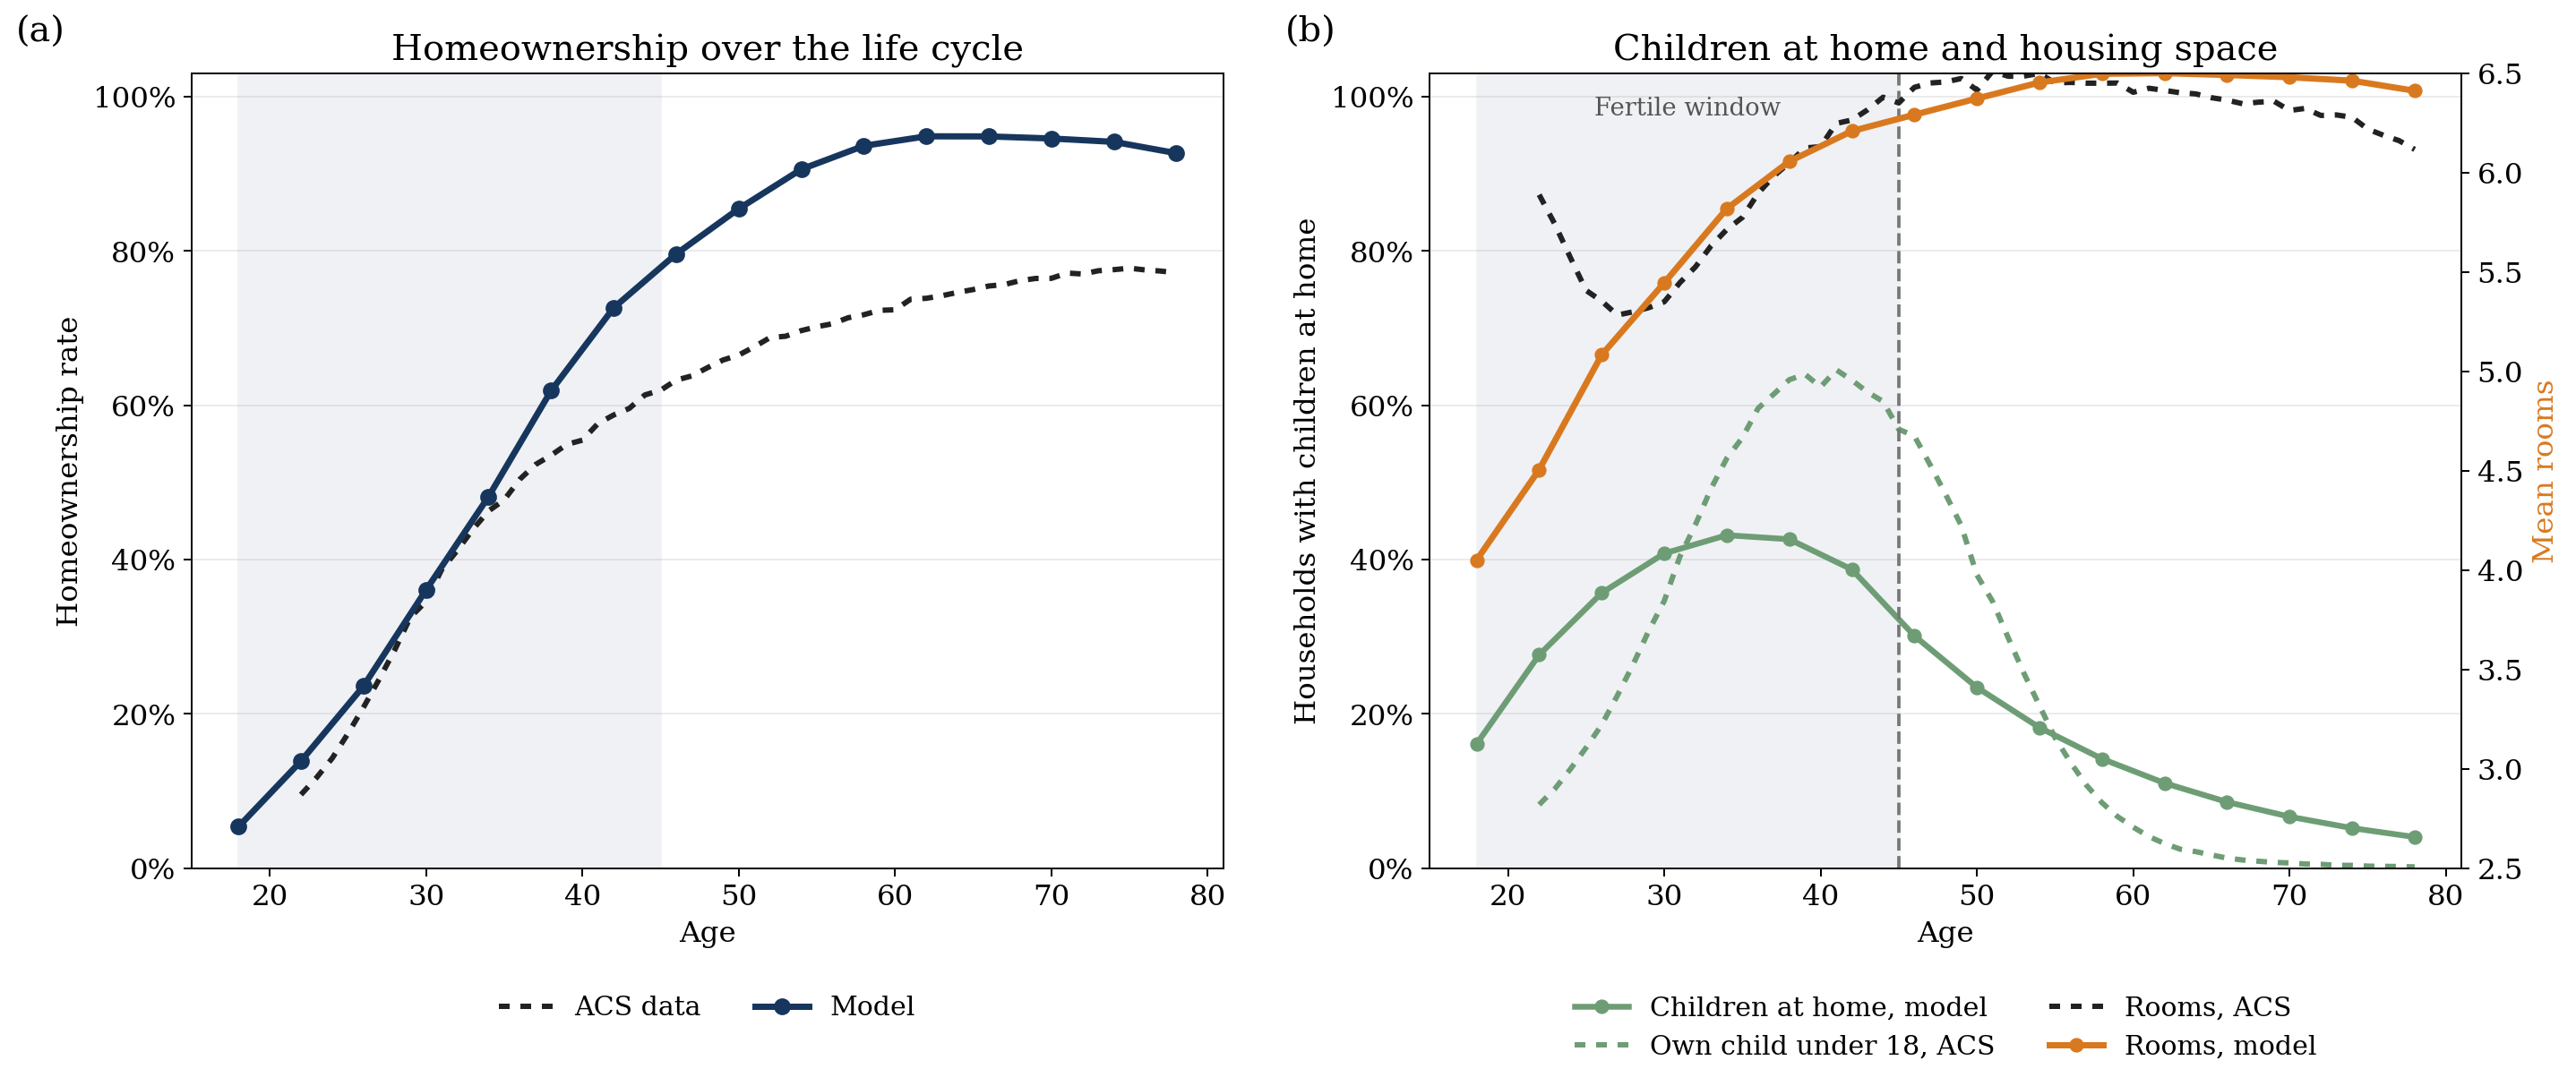
\includegraphics[width=0.98\textwidth]{eqscale_note_lifecycle_equilibrium.png}
\caption{Lifecycle ownership, children at home, and housing consumption at
the current estimate. Panel (a) compares model homeownership with the ACS
household-head profile. Panel (b) compares the model share of households with
dependent children at home with the ACS share of household heads with an own
child under age 18, and compares mean rooms in the model and the ACS. The
shaded region marks ages 18--45, the fertile window.}
\label{fig:eq_lifecycle}
\end{figure}

\begin{thebibliography}{9}

\bibitem[Borella et al.(2023)]{borellaDeNardiYang2023}
Borella, M., M. De Nardi, and F. Yang. 2023.
``Are Marriage-Related Taxes and Social Security Benefits Holding Back Female Labour Supply?''
\emph{Review of Economic Studies} 90(1): 102--131.

\bibitem[Davis and Van Nieuwerburgh(2015)]{davisHousingFinanceMacroeconomy2015}
Davis, M. A., and S. Van Nieuwerburgh. 2015.
``Housing, Finance, and the Macroeconomy.''
\emph{Handbook of Regional and Urban Economics} 5: 753--811.

\bibitem[De Nardi and Yang(2014)]{denardiYang2014}
De Nardi, M., and F. Yang. 2014.
``Bequests and Heterogeneity in Retirement Wealth.''
\emph{European Economic Review} 72: 182--196.

\bibitem[Flod\'en and Lind\'e(2001)]{flodenLinde2001}
Flod\'en, M., and J. Lind\'e. 2001.
``Idiosyncratic Risk in the United States and Sweden: Is There a Role for Government Insurance?''
\emph{Review of Economic Dynamics} 4(2): 406--437.

\bibitem[Gale and Scholz(1994)]{galeScholz1994}
Gale, W. G., and J. K. Scholz. 1994.
``Intergenerational Transfers and the Accumulation of Wealth.''
\emph{Journal of Economic Perspectives} 8(4): 145--160.

\bibitem[Greaney et al.(2025)]{greaneyDynamicUrbanEconomics2025}
Greaney, B., A. Parkhomenko, and S. Van Nieuwerburgh. 2025.
``Dynamic Urban Economics.'' Working paper.

\bibitem[Heathcote et al.(2017)]{heathcoteStoreslettenViolante2017}
Heathcote, J., K. Storesletten, and G. L. Violante. 2017.
``Optimal Tax Progressivity: An Analytical Framework.''
\emph{Quarterly Journal of Economics} 132(4): 1693--1754.

\bibitem[Leridon(2004)]{leridon2004}
Leridon, H. 2004.
``Can Assisted Reproduction Technology Compensate for the Natural Decline in Fertility with Age? A Model Assessment.''
\emph{Human Reproduction} 19(7): 1548--1553.

\bibitem[Saiz(2010)]{saizGeographicDeterminantsHousing2010}
Saiz, A. 2010.
``The Geographic Determinants of Housing Supply.''
\emph{Quarterly Journal of Economics} 125(3): 1253--1296.

\bibitem[Scholz et al.(2006)]{scholzSeshadriKhitatrakun2006}
Scholz, J. K., A. Seshadri, and S. Khitatrakun. 2006.
``Are Americans Saving `Optimally' for Retirement?''
\emph{Journal of Political Economy} 114(4): 607--643.

\end{thebibliography}

\end{document}
